Dos lados de un triángulo rectángulo miden 7 unidades y 3 unidades, como se muestra en la figura \ref{fig:area09}.
\begin{figure}[H]
    \begin{center}
        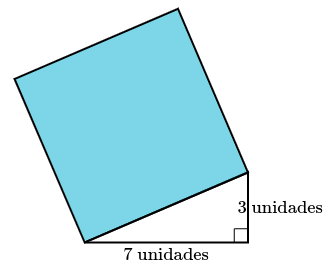
\includegraphics[width=0.4\textwidth]{../images/area09.png}
    \end{center}
    \caption{}
    \label{fig:area09}
\end{figure}
\textbf{¿Cuál es el área del cuadrado que comparte un lado con el tercer lado del triángulo?}